\documentclass{article}

\usepackage{graphicx}
\usepackage{hyperref}
\usepackage[english]{babel}
\usepackage{nameref}
\usepackage{caption}
\usepackage{float}

\begin{document}
	
	\begin{titlepage}
		\centering
		\vspace*{3cm}
		
		
\includegraphics[width=0.4\textwidth]{images/fontyslogo.png}
		\vspace{1.5cm}
		
		{\Huge\bfseries Prediction tool for mixed martial arts bout outcome}\\[1cm]
		
		\textbf{Danil Burov}\\
		\vspace{0.5cm}
		\textit{Fontys University of Applied Sciences}\\[3cm]
		\vfill
		\textbf{\today}
		
	\end{titlepage}
	\newpage
	\tableofcontents
	\newpage
\section{Introduction}
	The purpose of this document is to report in a comprehensive way all the work that has been done throughout my fifth semester regarding the creation of an AI tool for predicting the outcome of MMA bouts. To do so, I will explain each step that I took in order to deliver the final outcome of the project.
\section{Business understanding}
	%The different probabilities of bouts ending
	The primary objective of this project is to develop a predictive tool that provides insights into the outcome of a bout between two fighters. 
	Rather than offering a binary prediction (0 or 1, representing true or false outcomes), the tool generates probabilistic predictions on a scale 
	between 0 and 1. This allows users to understand the likelihood of various outcomes, such as the probability of a fighter submitting their opponent, 
	achieving a knockout, or winning by decision. By delivering granular insights, the tool empowers users to make data-driven assessments of match 
	outcomes.\\\\
	%Risk of gambling
	One notable risk associated with the project is its potential misuse for betting purposes. The tool could be exploited to gain unfair advantages in gambling
	scenarios. To mitigate this concern, the tool will be kept private and its access limited to legitimate and approved stakeholders.\\\\
	%Fighters' analytical tool
	Beyond the potential concerns, the tool holds immense value as an analytical resource for fighters and their coaching teams. Fighters can leverage
	the tool to analyze their strengths and weaknesses relative to their opponents. For instance, by understanding the likelihood of success in 
	specific fighting techniques, fighters can tailor their training regimens to exploit their opponent's vulnerabilities and address their own 
	shortcomings.

\section{Data understanding}
	The dataset selected for this project is sourced from Kaggle and contains data on every UFC fight from mid-2010 to the present. Each row in the dataset represents 
  an individual bout, making it well-suited for predictive modeling and analysis. This dataset was chosen for several reasons: it is regularly updated on a weekly basis
  , ensuring that the data remains current, and it already includes pre-processed statistics such as the difference in metrics between the two fighters in each bout. 
  Additionally, it provides key variables such as betting odds, fighter rankings, and fight statistics, as well as the target variable for this project, the bout
  "Winner." \\\\
  Despite its strengths, including over 6,000 entries and 118 features, there are still several limitations to consider regarding the accuracy and completeness of
  the model. Many critical factors that influence fight outcomes are not included in the dataset due to their subjective or difficult-to-quantify nature. 
  For example:\\\\
  \textbf{Mental State: }A fighter's psychological readiness, confidence, and focus leading up to the fight can significantly affect their performance. \\\\
  \textbf{Health Status: } Factors such as injuries, illnesses, or the general health of the fighter during training camp or on fight day are not accounted for.\\\\
  \textbf{Weight Cutting and Rehydration: } Many fighters undergo extreme weight cuts before weigh-ins, only to rehydrate and regain substantial weight before the fight. 
  The extent of their weight recovery and its impact on their physical condition during the bout is a crucial factor that is not captured in the dataset.\\\\
  Moreover, many day-to-day factors influencing a fighter's performance are inherently subjective and nearly impossible to gather systematically. Fighters
  themselves may not be fully aware of how these aspects—such as their recovery quality, nutrition, or emotional state—affect their performance in a bout.
  This lack of granular data presents a challenge in achieving high accuracy for predictive models.\\\\
  While these limitations highlight gaps in the dataset, they also underscore the opportunity for future research and data collection in combat sports. 
  If more detailed physiological and psychological data could be integrated into such datasets, it would pave the way for more accurate and robust predictive models
  in the domain of mixed martial arts.\\\\

  %Maybe add data visualizations here later after feedback
  %
 \section{Data preparation}
  %Refer to appendix most images
  In order to explain the data preparation done regarding the ufc dataset I will reference most of my explanations to the appendix. This was done to keep a neatly organized
  text. I will be using snippets from my Jupyter notebook. All these features are displayed here: \\
  \begin{figure}
    \centering
    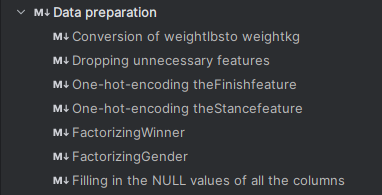
\includegraphics[width=0.8\textwidth]{images/ToC_Data_cleaning.png}
    \caption{Overview of data preparation processing steps}
  \end{figure}\\\\

  \subsection{Deleting columns}
 
  When the dataset was chosen it was known that many of the features will not be used for the purpose of the tool. All these features were dropped for a reason and in the 
  upcoming subsection it will be explained why. Initially the number of features was 118. After dropping the unnecessary features, the number was reduced to 49.\\\\ 
  These features were rankings, streak orientated, or keeping track of the fighters' decisions and win/lose streak, and other miscelanous features that are irrelevant.\\\\ 
  The code can be found below:\\
  	\begin{figure}[H]
  	\centering
  	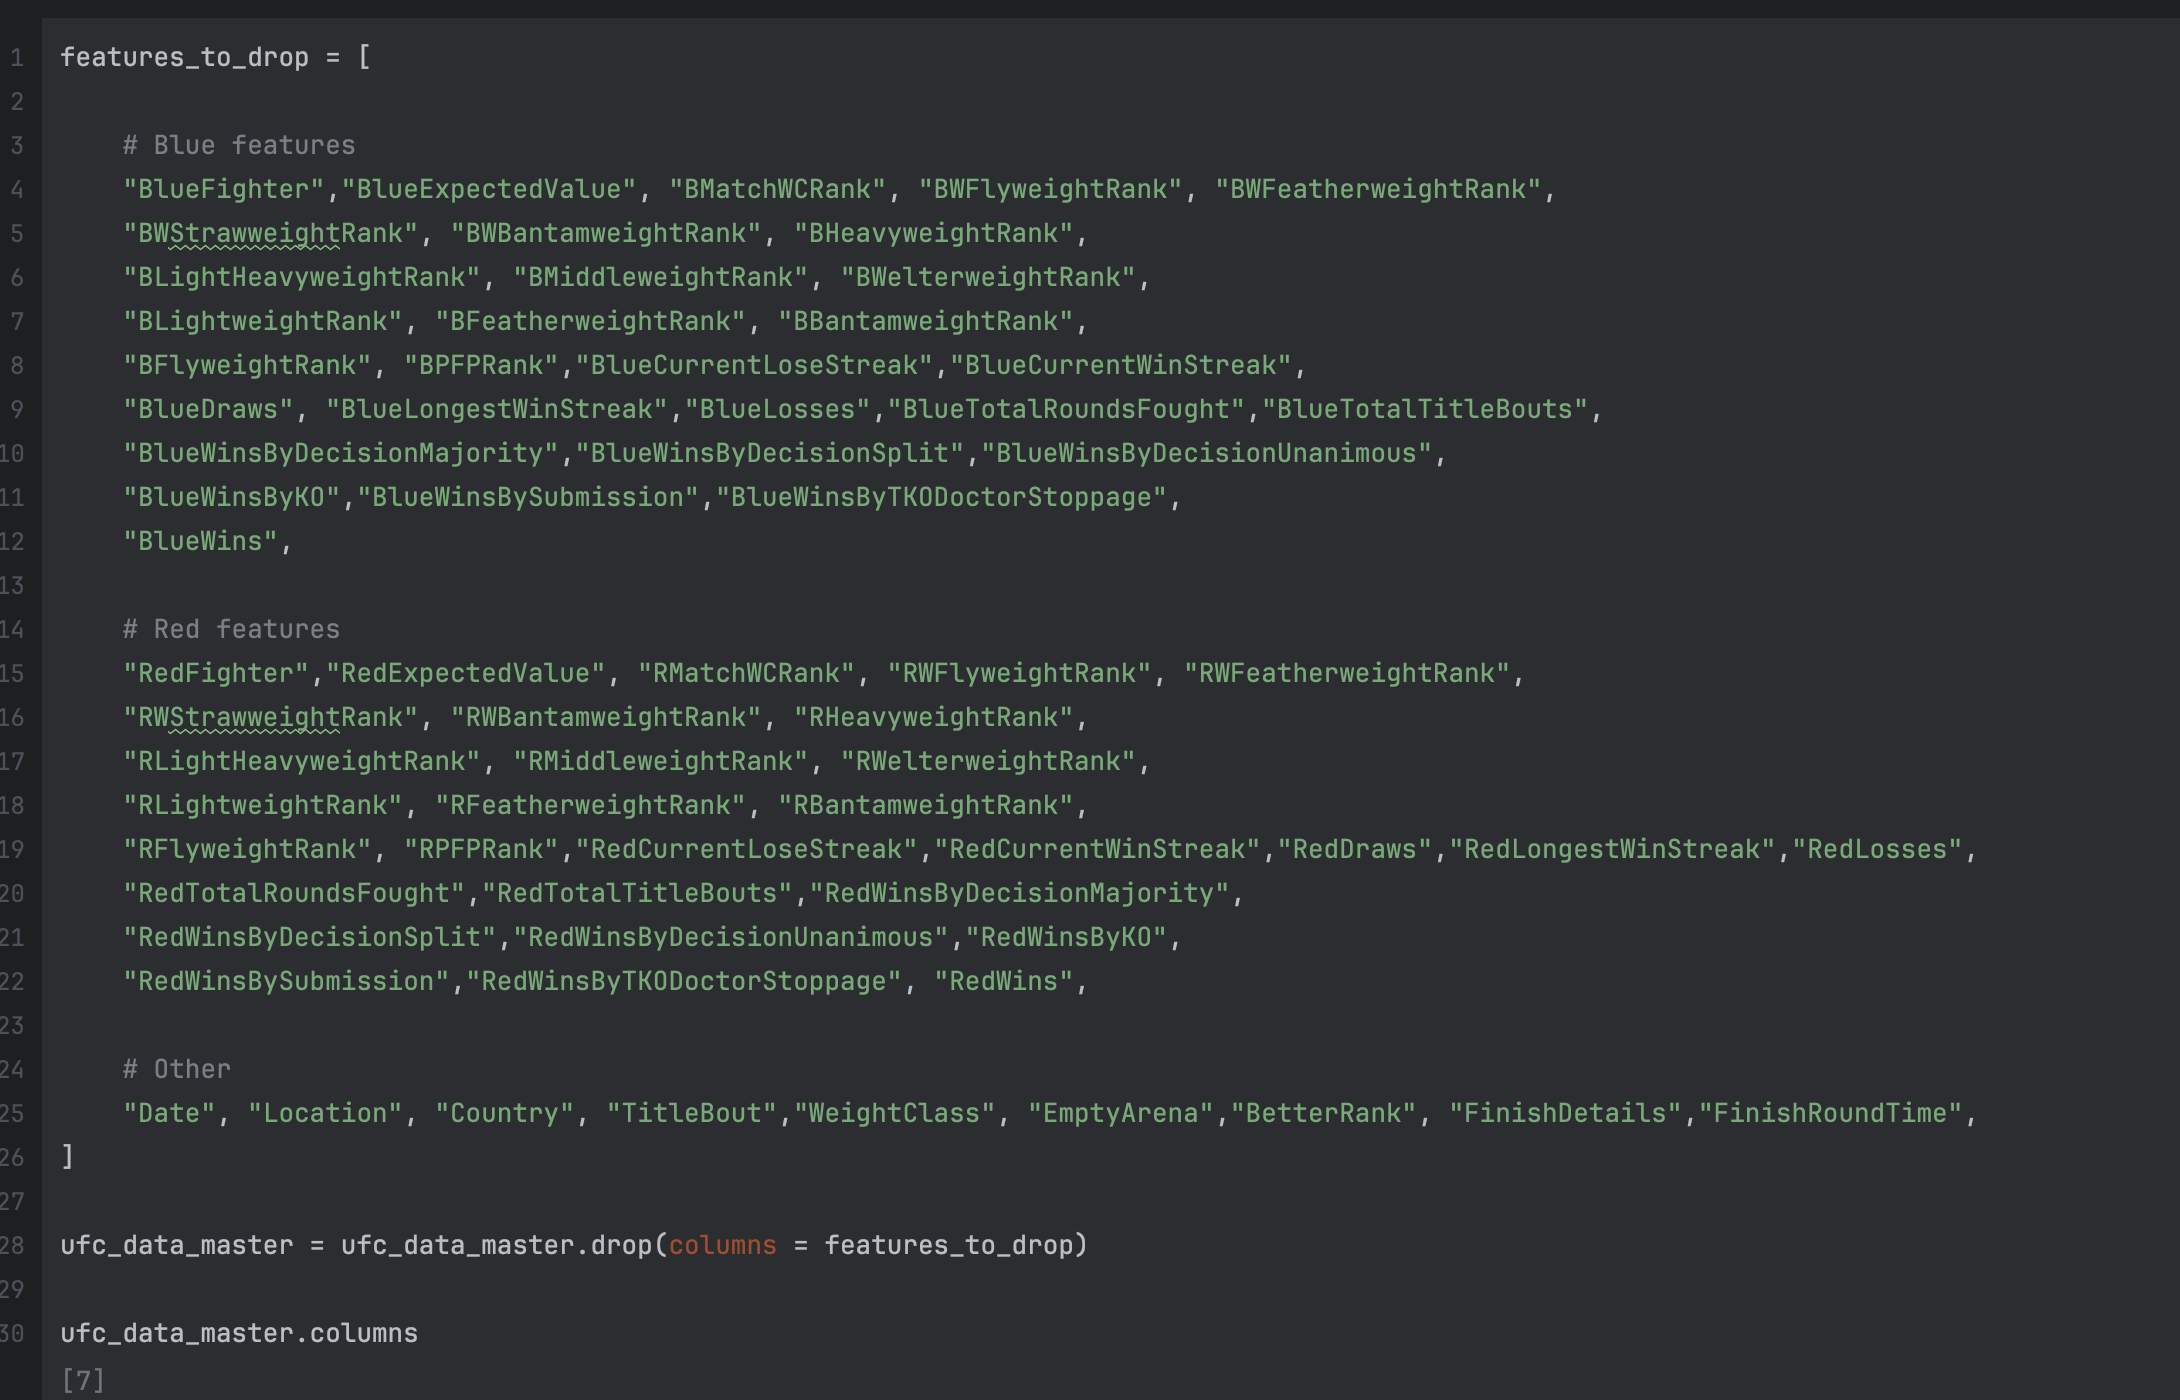
\includegraphics[width=1\textwidth]{images/Features_Dropped.png}
  	\caption{Unnecessary features dropped}
  \end{figure}
 \subsection{One-Hot-Encoding} %First explain what is one-hot-encoding, then explain why these features were one-hot-encoded and not factorized
  One-hot-encoding is used to trnasform categorical values into numberical values. In this case the 'Finish' feature had 5 different types of finished. When I one-hot-encode 
  the feature I get 5 different columns with all the possible finishes and every bout (each row in the dataset) has a true or false to the according finish. It is not a good idea 
  to factorize with that many different options because the model could develop bias towards the bigger numbers.\\\\ 
  One-hot-encoding was used not only to encode the 'Finish' feature but also the 'Stance' feature. 'Stance' had three possible values 'Southpaw', 'Ortohodox', 'Switch'.\\\\
  The code for one-hot-encoding the 'Finish' feature can be found:\\
\begin{figure}[H]
	\centering
	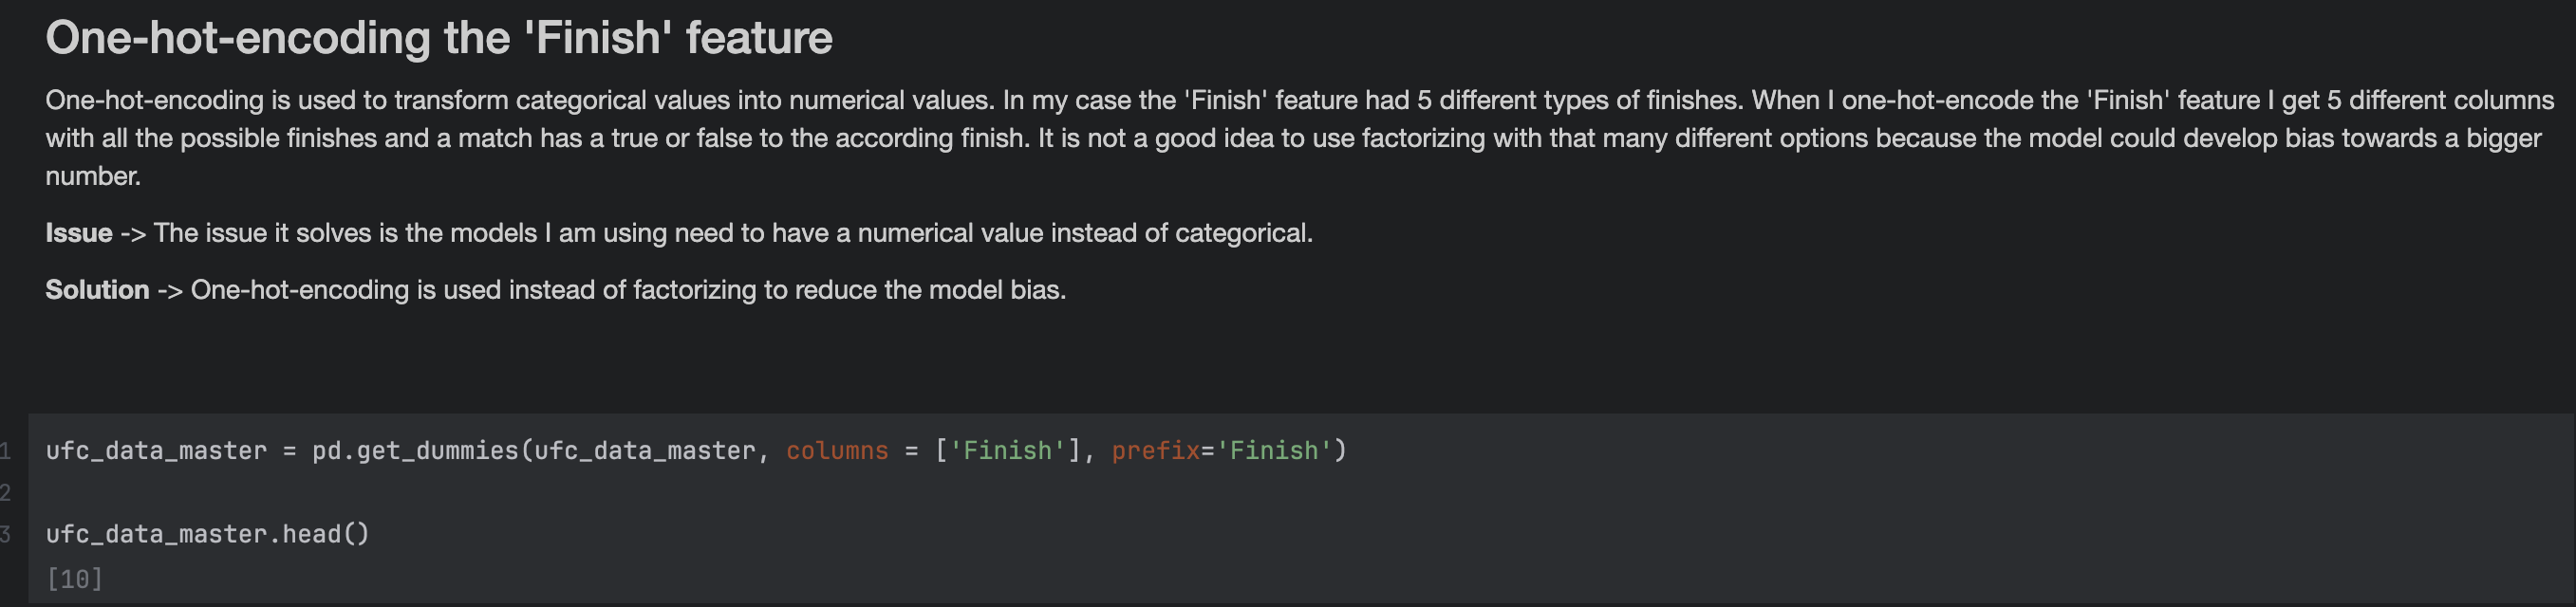
\includegraphics[width=1\textwidth]{images/One_hot_encoding_finish.png}
	\caption{One-Hot-Encoding 'Finish' feature}
\end{figure}
  The code for one-hot-encoding the 'Stance' feature can be found below:\\
  \begin{figure}[H]
  	\centering
  	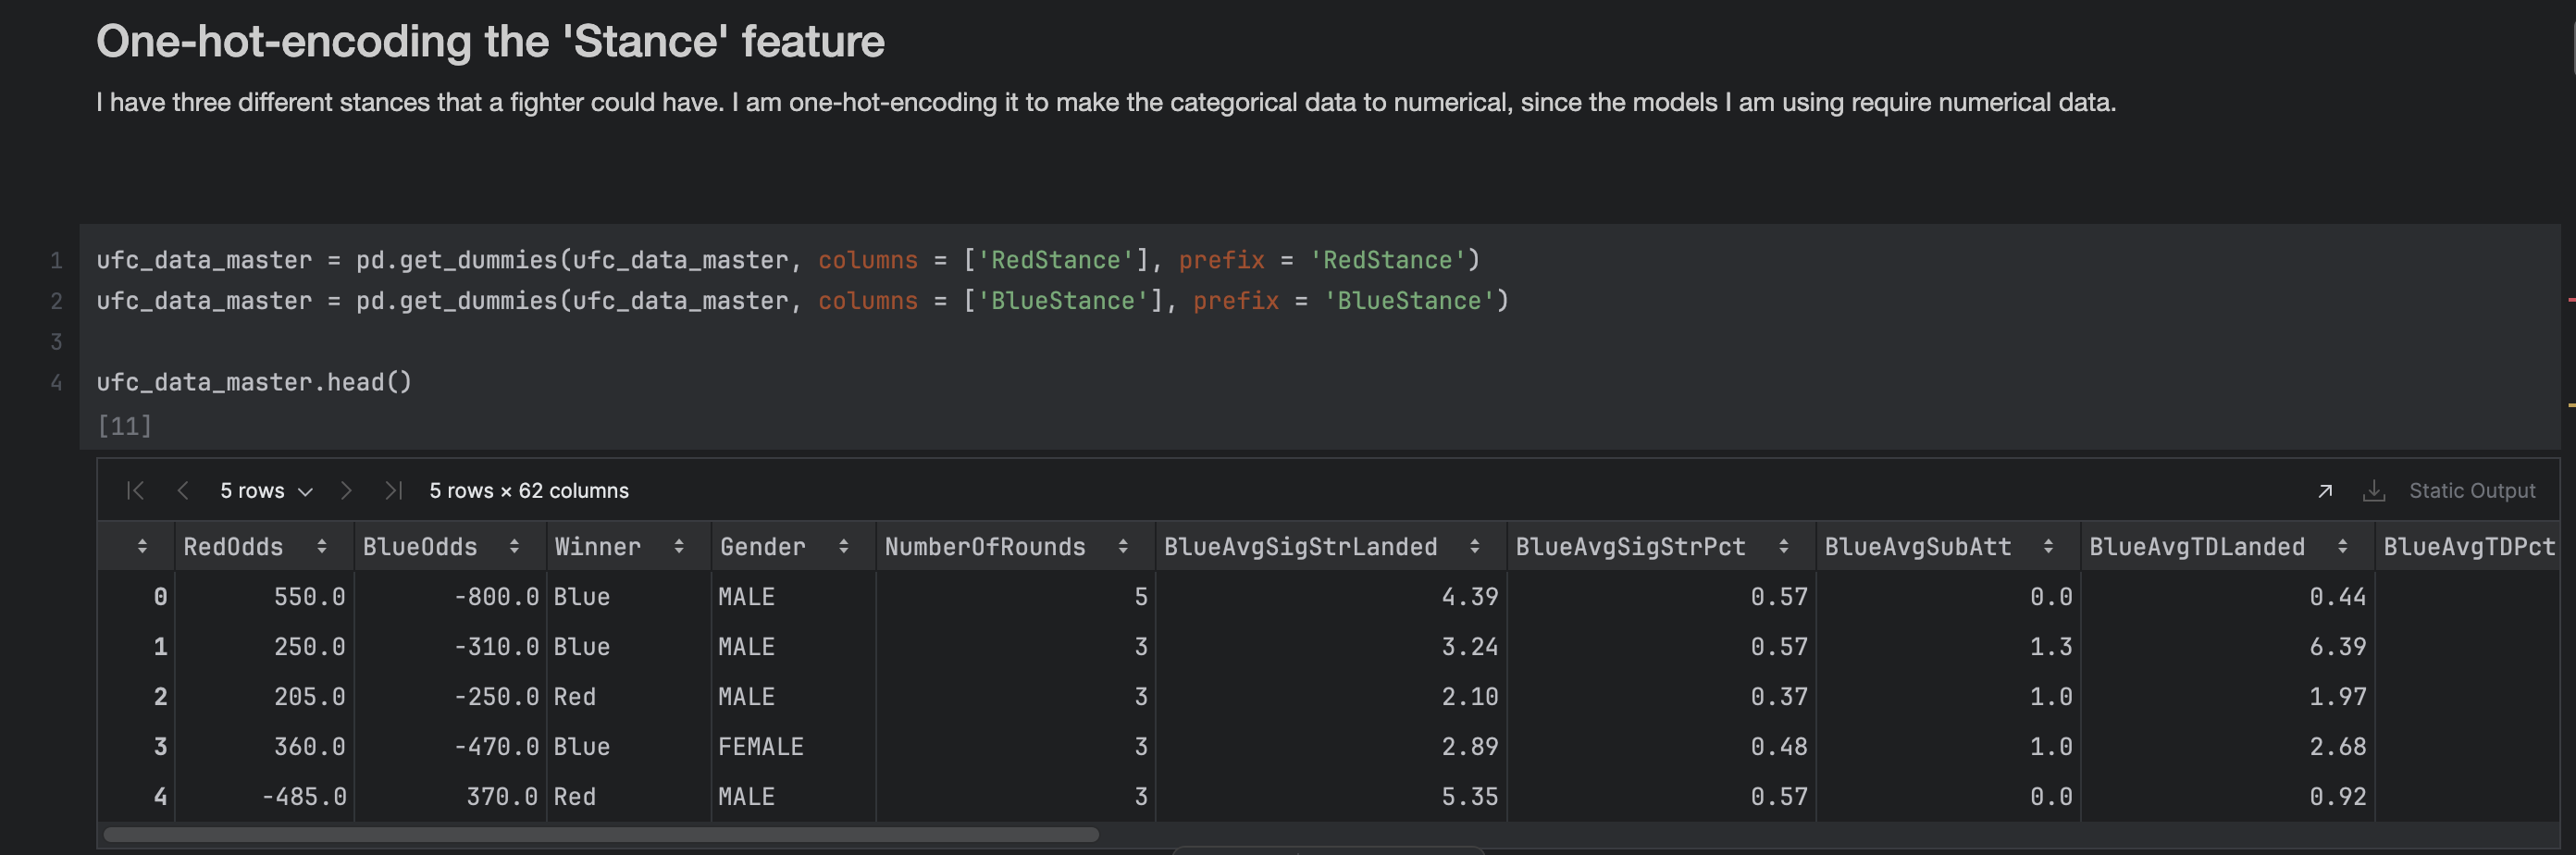
\includegraphics[width=1\textwidth]{images/One_hot_encodiong_Stance.png}
  	\caption{One-Hot-Encoding 'Stance' feature}
  \end{figure}
  \subsection{Scalling}
  In general all the features in the dataset need to be scalled to standard deviation. That is the reason why all the features that had percentage were scalled to a decimal to the first zero.\\\\ 
  Additionally I converted the 'Weight' feature from LBS to KG, because it is more convenient for me. \\\\
  The code can be found below:\\
  \begin{figure}[H]
  	\centering
  	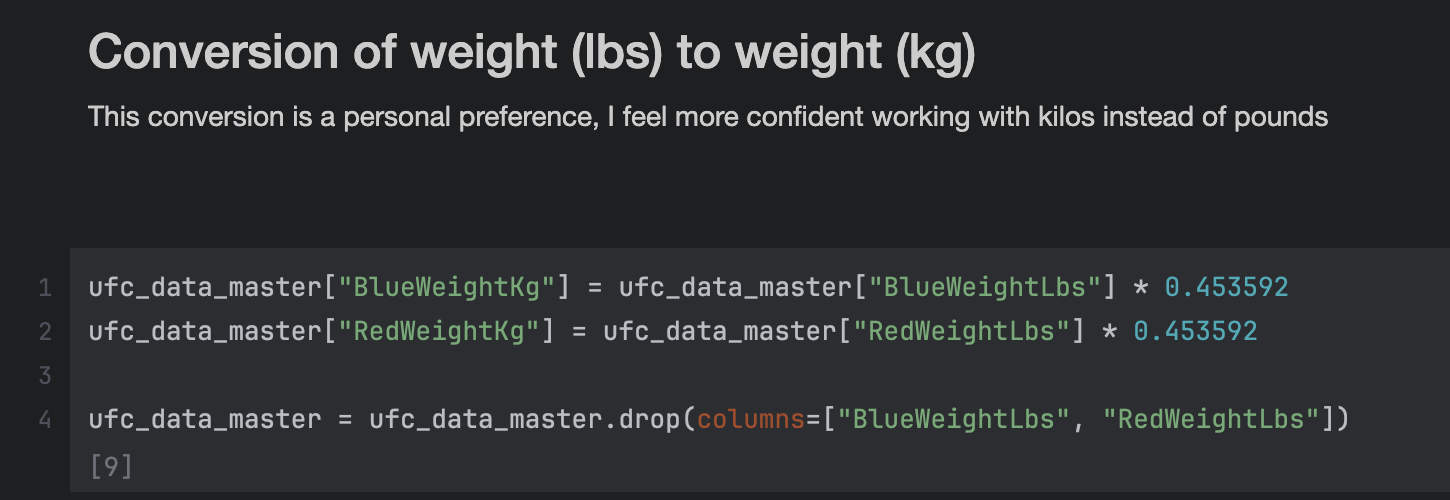
\includegraphics[width=1\textwidth]{images/Conversion_weight_lbs_to_kg.png}
  	\caption{Converting the 'Weight' feature from lbs to kg}
  \end{figure}
  \subsection{Factorzing}
  For some features one-hot-encoding is not exactly needed. In this case it was decided to factorize values that can have only two possible values. However in some cases 
  it could be better to even use one-hot-encoding with these features as well because some models can deal with more features more efficiently. The reason these features were 
  factorized is because in the beginning the project was supposed to train a classification model where the output is either 0 or 1, however the idea changed but factorizing is still 
  good enoigh for the model that is currently being used.\\\\ 
  Since the dataset contains both genders the feature that was factorized is the 'Gender' where the 0 is \underline{man} and the 1 is a \underline{woman}.\\\\
  Another feature that has only two values is the 'Winner' feature, which has either red or blue, depending on who won the fight (Red and Blue are universal colours used to indicate the 
  corner that fighter fought from.). When factorized, 0 corresponds to \underline{Red} and 1 corresponds to \underline{Blue}. \\\\ 
  Code for factorizing the 'Gender' feature can be found below:\\
  \begin{figure}[H]
  	\centering
  	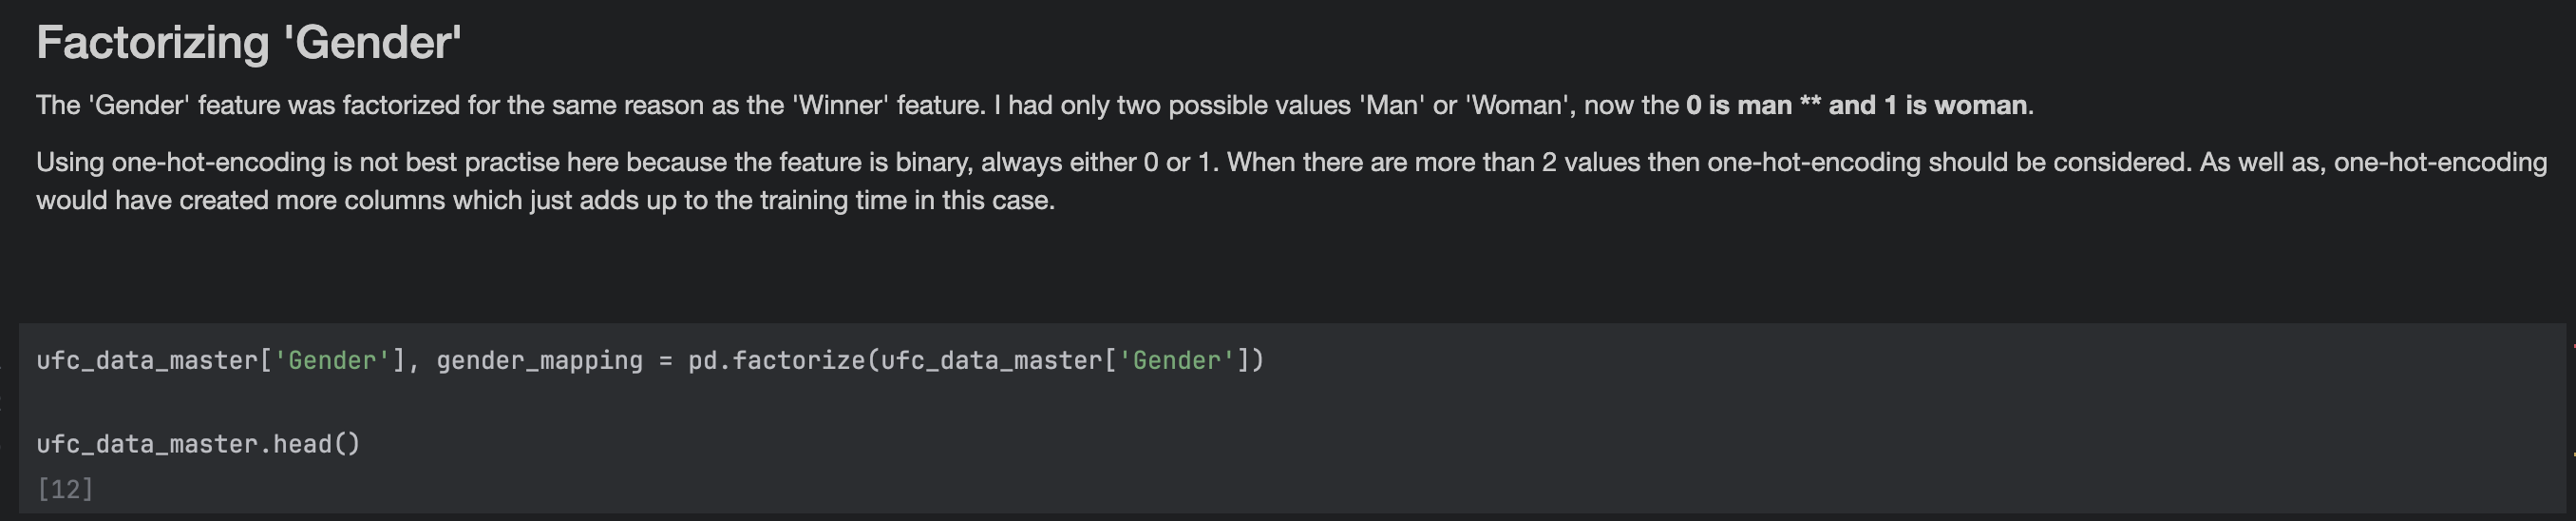
\includegraphics[width=1\textwidth]{images/Factorizing_Gender.png}
  	\caption{Factorizing the 'Gender' feature}
  \end{figure}
  Code for factorizing the 'Winner' feature can be found below:\\
  \begin{figure}[H]
  	\centering
  	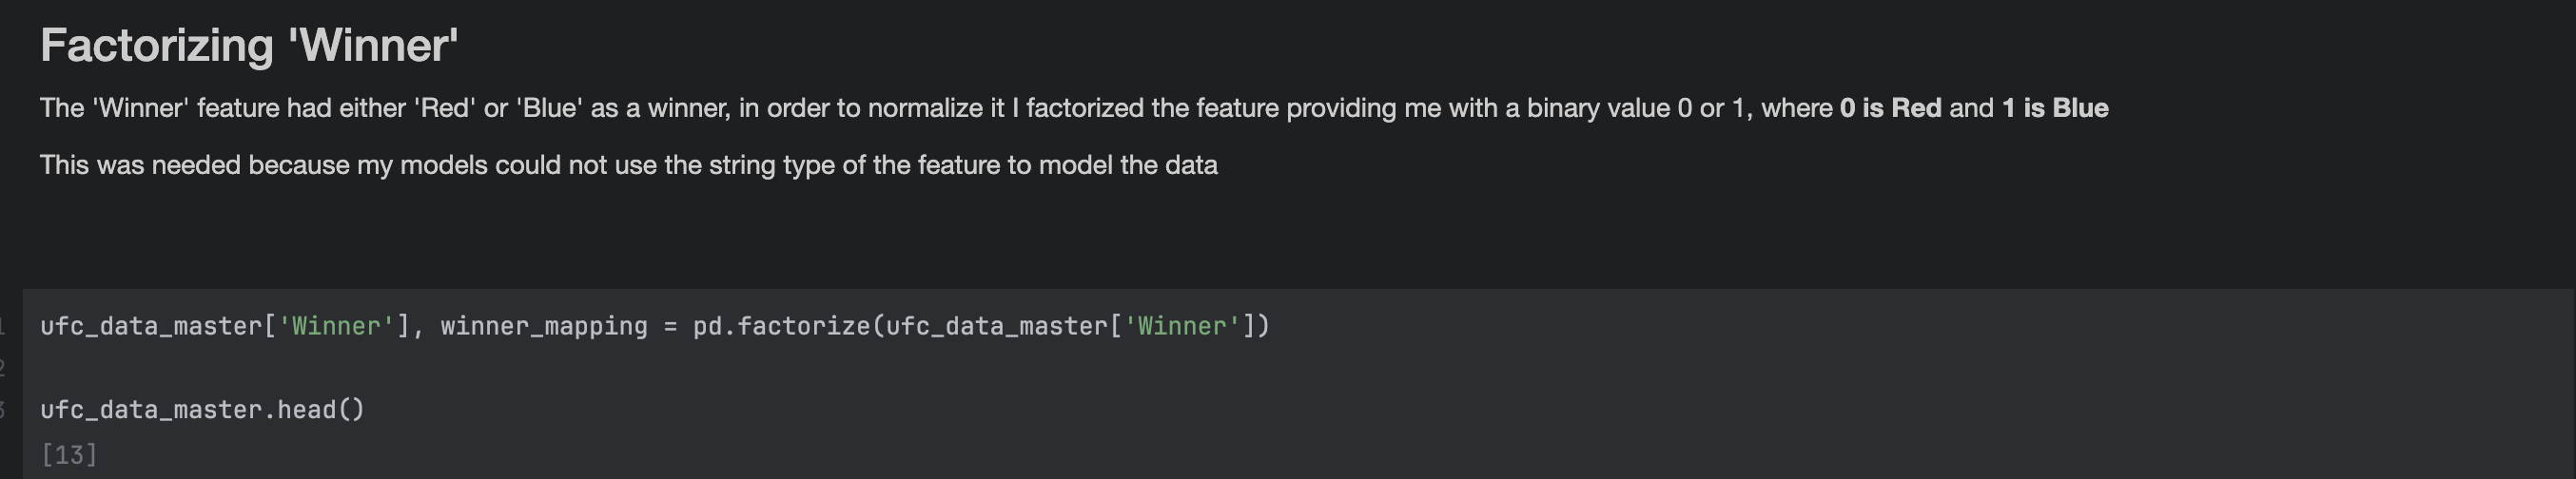
\includegraphics[width=1\textwidth]{images/Factorizing_Winner.png}
  	\caption{Factorizing the 'Winner' feature}
  	\label{fig:factorizing_winner}
  \end{figure}
  \subsection{Filling NaN values}
  The dataset has \textbf{415296} total entries from all features from which \textbf{19601} are NULL values. There were three options how to deal with all the different values. 
  First was to fill in the missing values with 0 or specific string text wherever is needed. Second was to delete the rows that had these NULL values. However, 
  the condition for this is the rows that are missing values to be less than 10 percent. And the last possible action was to develop a ML model that feels in these 
  values. This option was not developed. \\\\ 
  Most of the features did not have a significant impact on the accuracy of the model that is why they were filled with 0. Most of the rows that had NULL features were both from the 
  red and blue corner (e.g. The 'RedOdds' feature and 'BlueOdds' feature in the row were both NULL so filling them with 0 just fixes the empty value)\\\\ 
  Code for filling the NaN values can be found below:
  \begin{figure}[H]
  	\centering
  	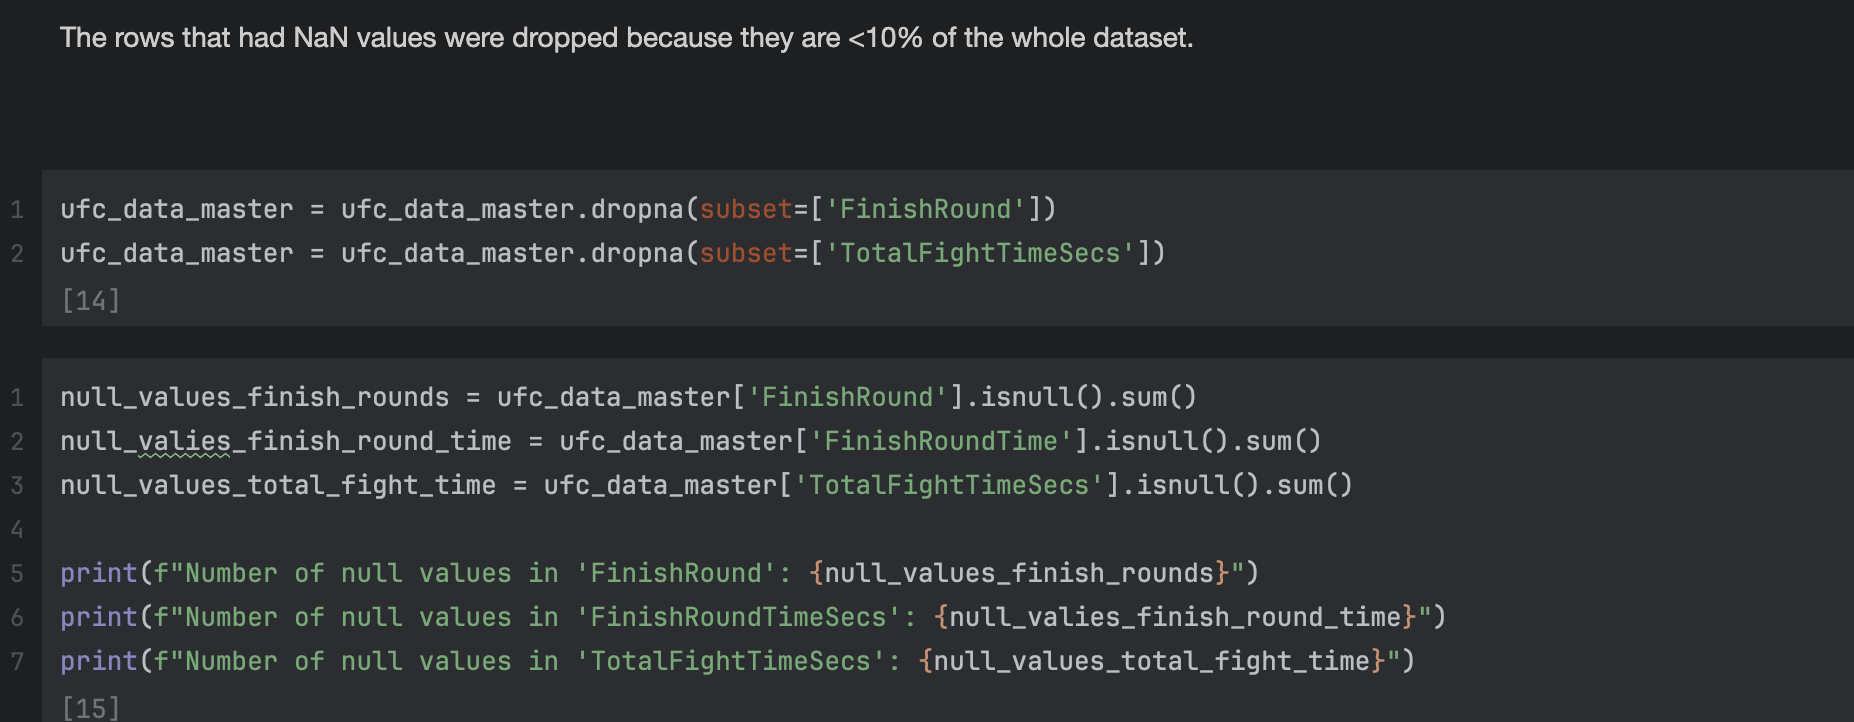
\includegraphics[width=1\textwidth]{images/Filling_NaN_Values.png}
  	\caption{filling the NaN values}
  	\label{fig:filling_nan_values}
  \end{figure}
\section{Modelling}
Choosing a model for the data was difficult given the reason that the project idea was to not predict if a fighter is going to win (0 or 1), but rather see the likelihood of a fighter winning in three different outcomes against the opponent. Knowing this, logistic regression seemed like a good fit for the project.\\\\
Logistic regression under the hood is a classification model that uses the Sigmoid function. Although, given its classification nature, it provides the probability output between 0 and 1.\\\\
In this project, four different models were trained with the data. This is due to the fact that the target variable needed to be existent in the dataset. In the beginning, an imaginary target variable was created, which was a combination of all the targets: 'Winner', 'Finish\_KO/TKO', 'Finish\_SUB', 'Finish\_U-DEC'. For this project, other finishes were not taken into account for simplicity reasons. Although further development could be the prediction of the rest finish outcomes of a match, e.g., 'Doctor stoppage'.\\\\
Four different baseline models were trained for the purpose of the project. Each one having the according target variable. The winner prediction model has a baseline accuracy of \textbf{0.62\%}, the KO/TKO has \textbf{0.67\%}, submission has \textbf{0.80\%}, and the unanimous decision model has \textbf{0.66\%} accuracy. However, looking into the confusion matrixes of all the models it was easily established that the model has a big bias towards the blue corner.
Below will be displayed the confusion matrixes of all the baseline models.\\\\
\newpage
	{\large \textbf{Winner baseline model}}\\\\
	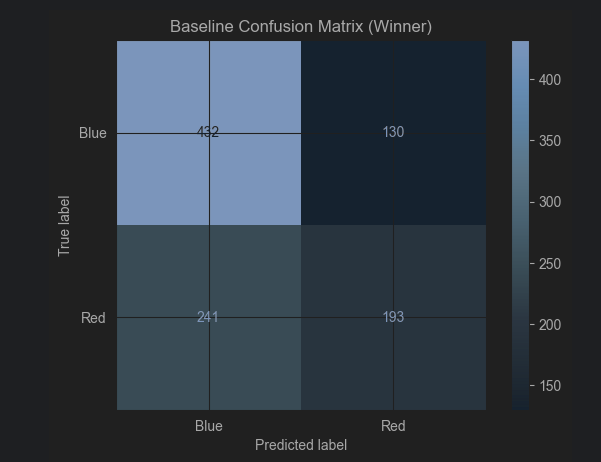
\includegraphics[width=0.5\textwidth]{images/CM_Winner.png}\\\\
	
	{\large \textbf{Finish\_KO/TKO baseline model}}\\\\
	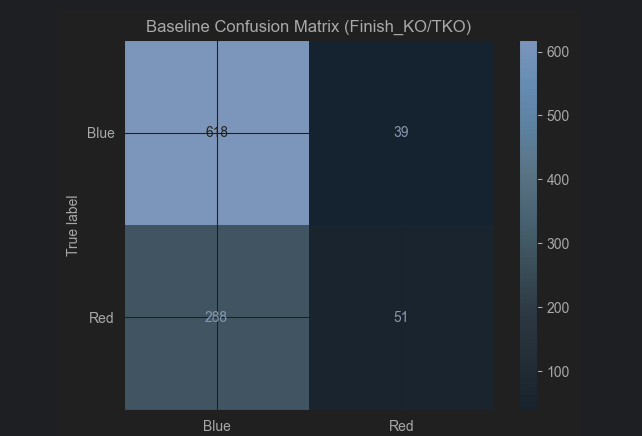
\includegraphics[width=0.5\textwidth]{images/CM_KO-TKO.png}\\\\
	\newpage
	{\large \textbf{Finish\_SUB baseline model}}\\\\
	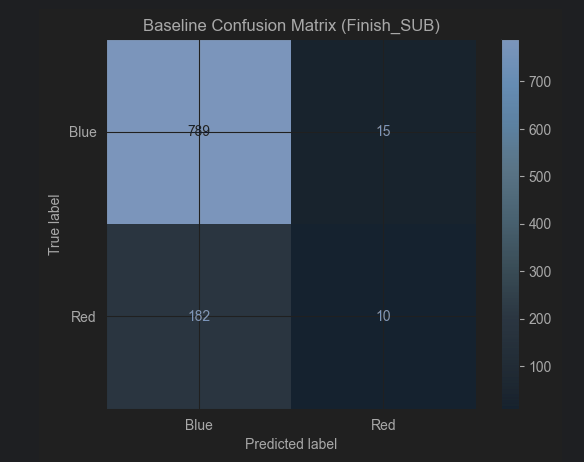
\includegraphics[width=0.5\textwidth]{images/CM_Submission.png}\\\\
	
	{\large \textbf{Finish\_U-DEC baseline model}}\\\\
	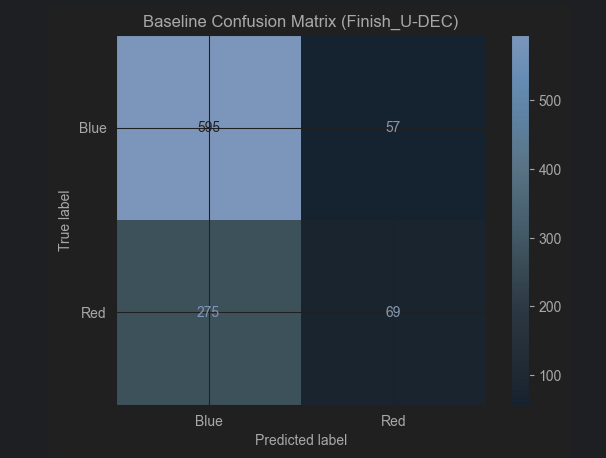
\includegraphics[width=0.5\textwidth]{images/CM_U-DEC.png}\\\\
	
It is very clear that the models are not really predicting well. All of them seem to have some sort of bias towards the blue fighter and they are mainly predicting if the blue fighter will win and they cannot predict that well if a red fighter will win.

\subsection{Optimization}
Logistic regression was used to train four models with four different target variable. However on all of them this bias towards the blue corner was persistent. In order to mitigate this bias, balancing the set was needed. Hyperparameter tuning, oversampling and undersampling were performed on the datasets and then the data was trained again using Logistic regression. For all models it seemed that oversampling worked best for balancing the set, however regarding accuracy it wasn't always the best pick.
Below I will showcase all the balancing results for all four models.
\newpage


	{\large \textbf{Hyperparameter Tuning Score - Winner}}\\\\
	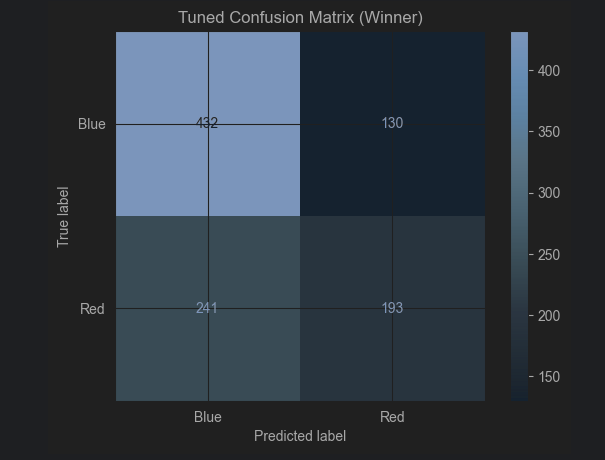
\includegraphics[width=0.5\textwidth]{images/CM_Hyp_Winner.png}\\\\

	{\large \textbf{Oversampling/Undersampling Score - Winner}}\\\\
	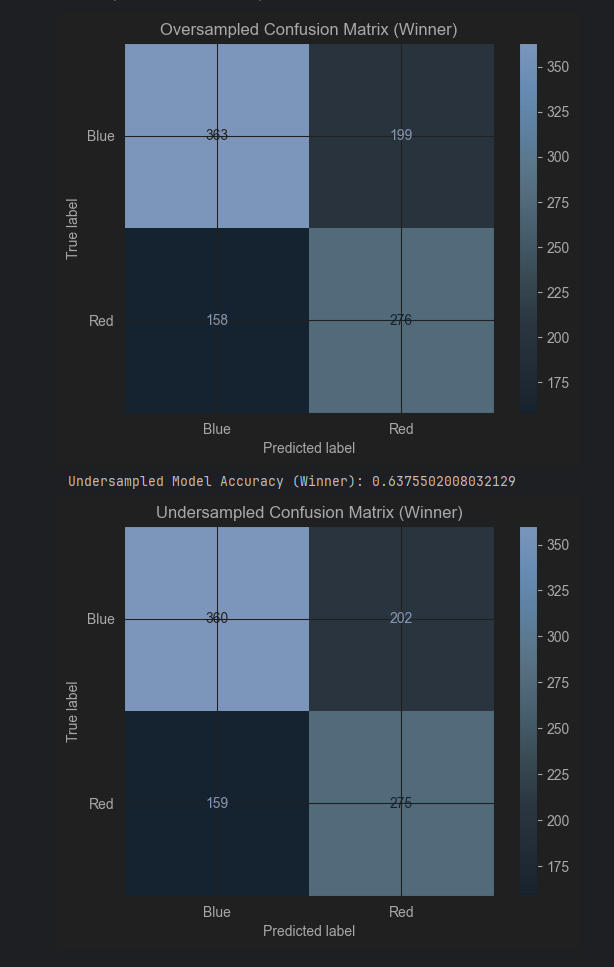
\includegraphics[width=0.5\textwidth]{images/CM_U_O_Win.png}\\\\
	In this model, hyperparameter tuning and balancing the set results in a better prediction after all. It is seen that in the oversampling technique the confusion matrix shows a better prediction when it comes to red winners, however with a trade-off for more false predictions on the blue side.
	
	{\large \textbf{Hyperparameter Tuning Score - Finish\_KO/TKO}}\\\\
	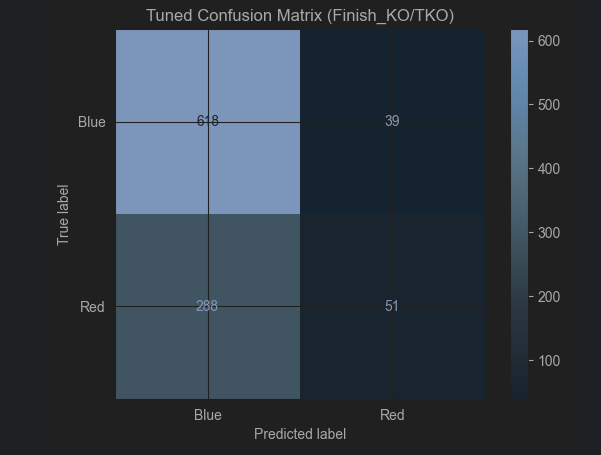
\includegraphics[width=0.5\textwidth]{images/CM_Hyp_KO-TKO.png}\\\\
	{\large \textbf{Oversampling/Undersampling Score - Finish\_KO/TKO}}\\\\
	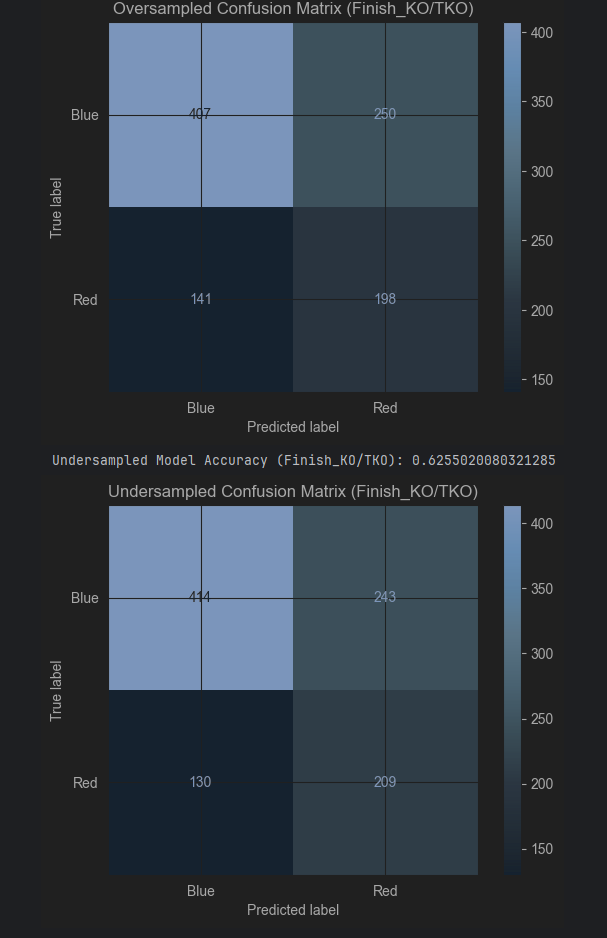
\includegraphics[width=0.5\textwidth]{images/CM_U_O_KO-TKO.png}\\\\
	Here the techniques applied do not result in a favourable result. Although, using oversampling did increase the true predictions for red, they are still quite low and the prediction is not reliable.
	\newpage
	{\large \textbf{Hyperparameter Tuning Score - Finish\_SUB}}\\\\
	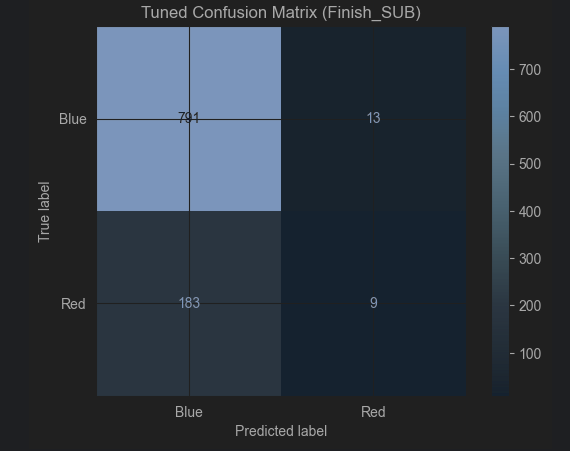
\includegraphics[width=0.5\textwidth]{images/CM_Hyp_SUB.png}\\\\
	{\large \textbf{Oversampling/Undersampling Score - Finish\_SUB}}\\\\
	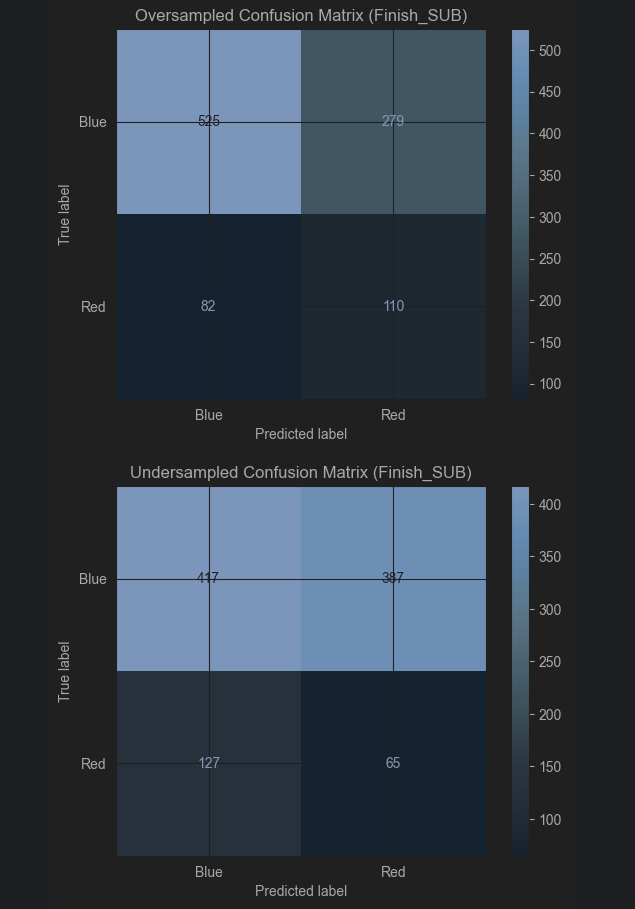
\includegraphics[width=0.5\textwidth]{images/CM_U_O_SUB.png}\\\\
	Unfortunately, this is the worst predicting model. There is an exponentially high bias towards the blue fighter and even with balancing of the set the bias is still too high.
	\newpage
	{\large \textbf{Hyperparameter Tuning Score - Finish\_U-DEC}}\\\\
	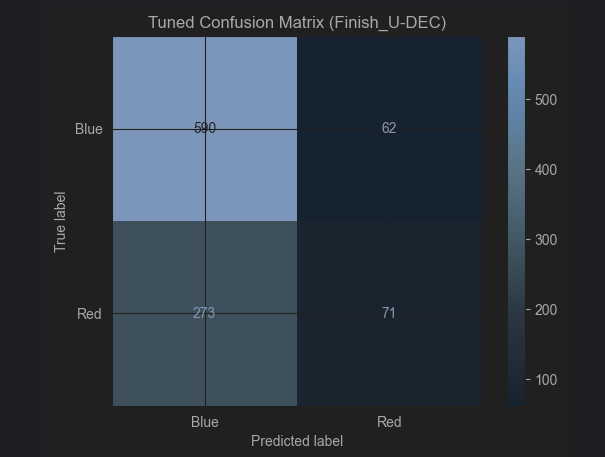
\includegraphics[width=0.5\textwidth]{images/CM_Hyp_U-DEC.png}\\\\
	{\large \textbf{Oversampling/Undersampling Score - Finish\_U-DEC}}\\\\
	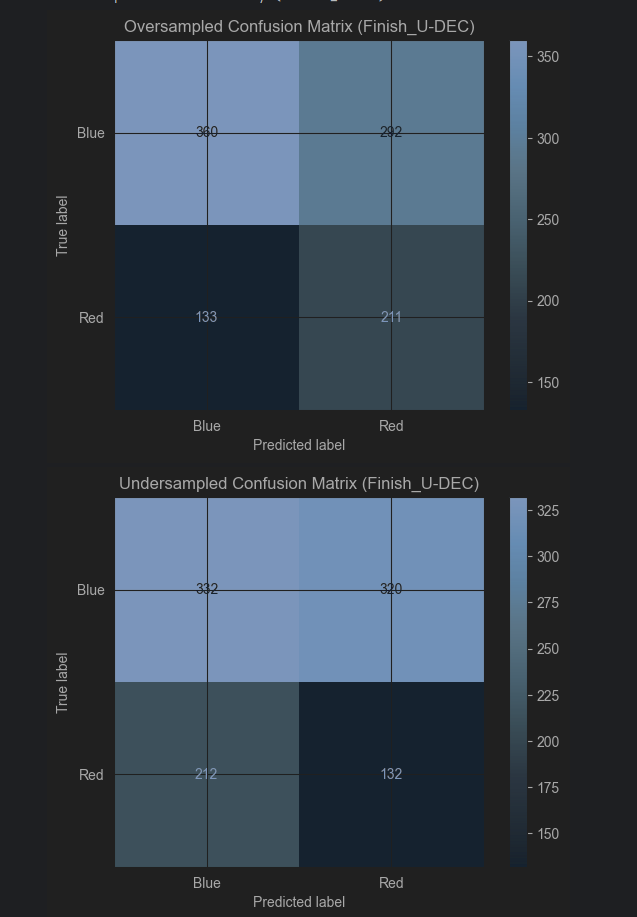
\includegraphics[width=0.5\textwidth]{images/CM_U_O_U-DEC.png}\\\\
	This model has the same outcome as the submission model. It just does not perform well at all. Based on the confusion matrixes it is seen that there is an even distribution of true - positivies and true-negatives which is absolutely incorrect.
	\newpage
	It is very clear that hyperparameter tuning doesn't really boost the performance of the model. The model is still predicting blue fighters better than red fighters, however the accuracy in some of the cases does increase.\\
	Opposed to oversampling which boosts the fairness of the model on all of the models. This is due to the fact that the oversampling technique populates the minority class (blue) with synthetic data. However this should be taken with a grain of salt because the synthetic data could be duplicates which might influence the models' accuracy and prediction.
\section{Conclusion}
Overall, the baseline models are very insufficient and if the model is to be used in any way it needs to have a more balanced set due to the difference between the red and blue winners in the dataset. It makes it so that the dataset develops a bias towards a winner. However, there is at least one good model from each outcome. The highest score of accuracy was achieved in the following optimized models: oversampled winner models with accuracy \textbf{0.64\%}, hyperparameter tuned finish\_ko/tko model with accuracy \textbf{0.67\%}, hyperparameter tuned submission model with \textbf{0.80\%}, baseline model for the unanimous decision model \textbf{0.66\%}.It is very difficult to predict an outcome of a match or which fighter will win. There are many attributes that need to be taken into account. There is a possible further continuation of the project, looking into betting odds. I personally think that this could be a good direction of the project.\\
\end{document}
